\lstset{backgroundcolor = \color{lightgray!20},
  basicstyle=\ttfamily,
  keywordstyle=\color{blue}\ttfamily,
  stringstyle=\color{red}\ttfamily,
  commentstyle=\color[HTML]{31B404}\ttfamily,
  language = Matlab
}

\section{Annotated code}

The Matlab code here is taken from the website: \url{http://cvlab.epfl.ch/software/daisy}.
As said in the code documentation, the code is divided into precomputation and
descriptor computation steps.

\subsection{Compute histograms for each pixel}

The histograms are computed in the precomputation step, ie.\ in the
\textbf{init\_daisy} function.

\begin{lstlisting}
%% compute histograms
h = size(im,1);
w = size(im,2);
for r=1:cn
    dzy.TCL(:,:,:,r) = transpose_cube(dzy.CL(:,:,:,r));
    dzy.H(:,:,r) = reshape( dzy.TCL(:,:,:,r), h*w, HQ );
end
\end{lstlisting}

The variable \textbf{dzy.CL} contains the ``cubes'' of the image. A cube means
the scale-space representation. The variable \textbf{HQ} is the number of bins
in the histogram.

For reference, here's the \textbf{transpose\_cube} function.
\begin{lstlisting}
function tc = transpose_cube( cube )
[h, w, n]=size(cube);
tc(w,h,n)=single(0);
for i=1:n
    tc(:,:,i) = transpose(cube(:,:,i));
end
\end{lstlisting}

\subsection{Normalize histograms to unit norm}

In the code, normalization seems to be done as the last step, after the
descriptor has been computed.

By default, the code uses partial normalization.
\begin{lstlisting}
function dsc = normalize_partial(udsc)

gn = size( udsc,1 );
dsc = udsc;
for i=1:gn
    n = norm(udsc(i,:));
    if n~= 0, dsc(i,:) = udsc(i,:)/n; end
end
\end{lstlisting}


\subsection{DAISY descriptor is computed}

\section{Directional derivative images}

\begin{figure}\label{fig:face}
  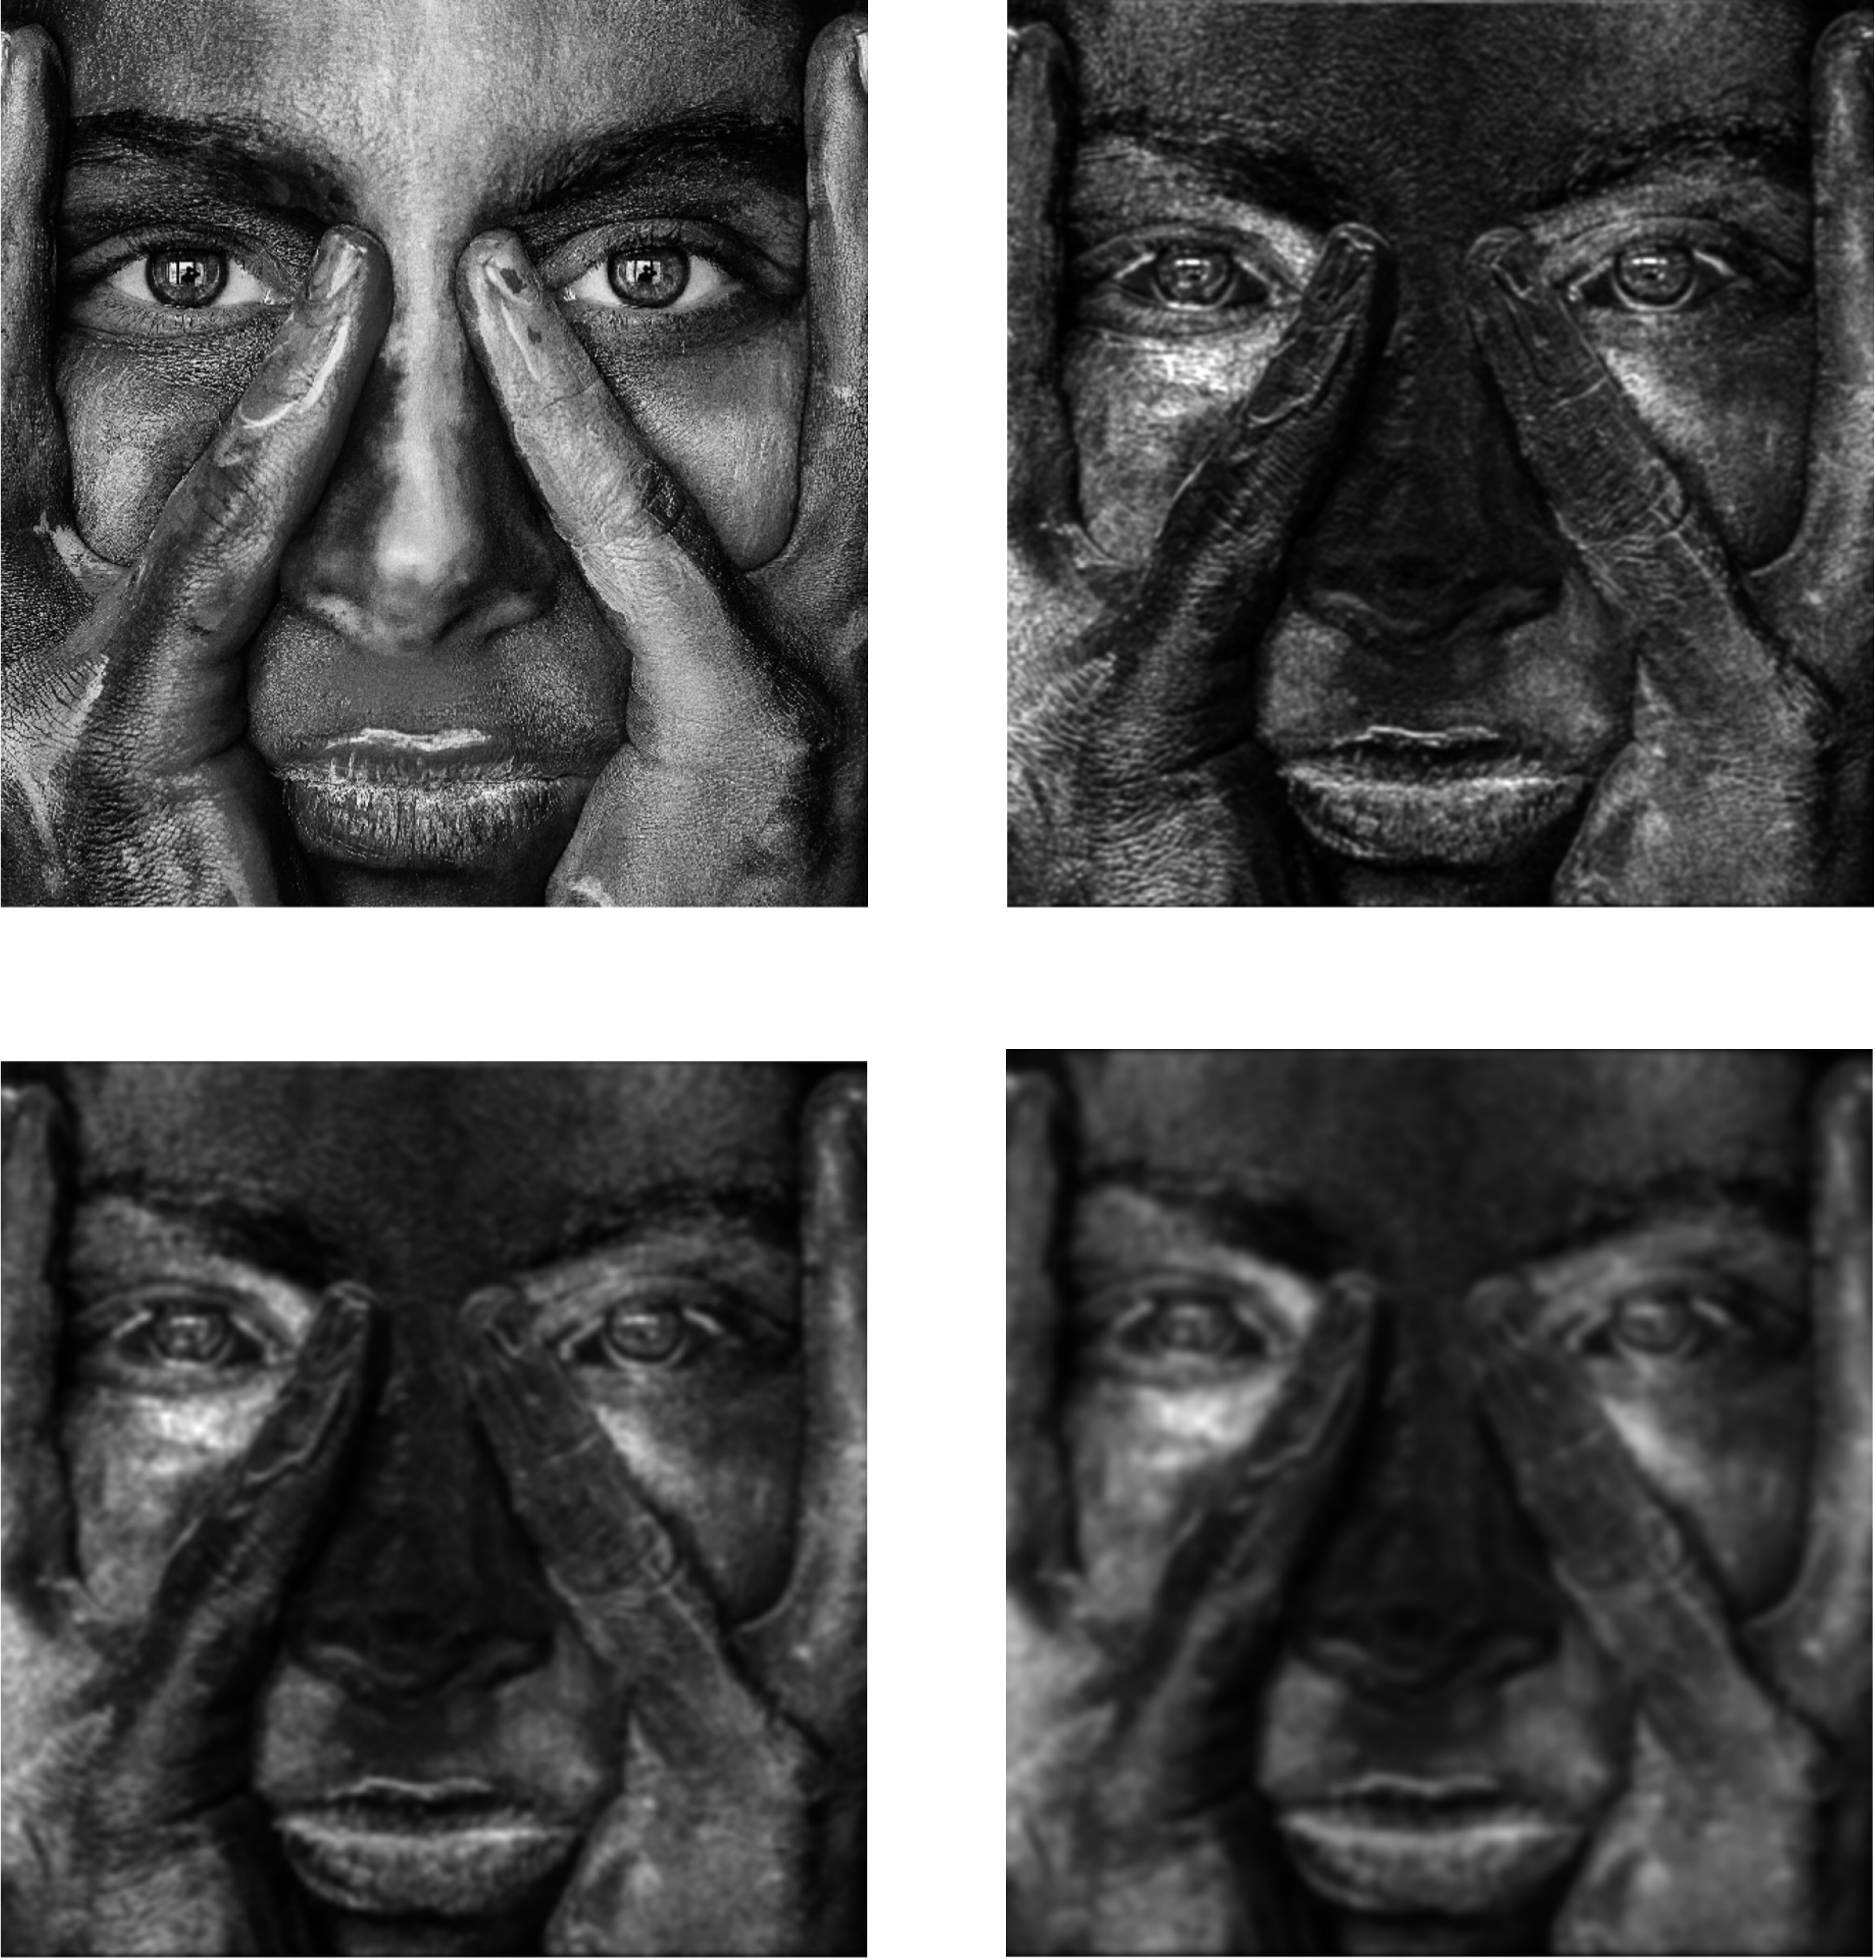
\includegraphics[width=\textwidth]{image1-table}
  \caption{Three directional derivative images and the original in the top-left
  corner}
\end{figure}

\begin{figure}\label{fig:grasshopper}
  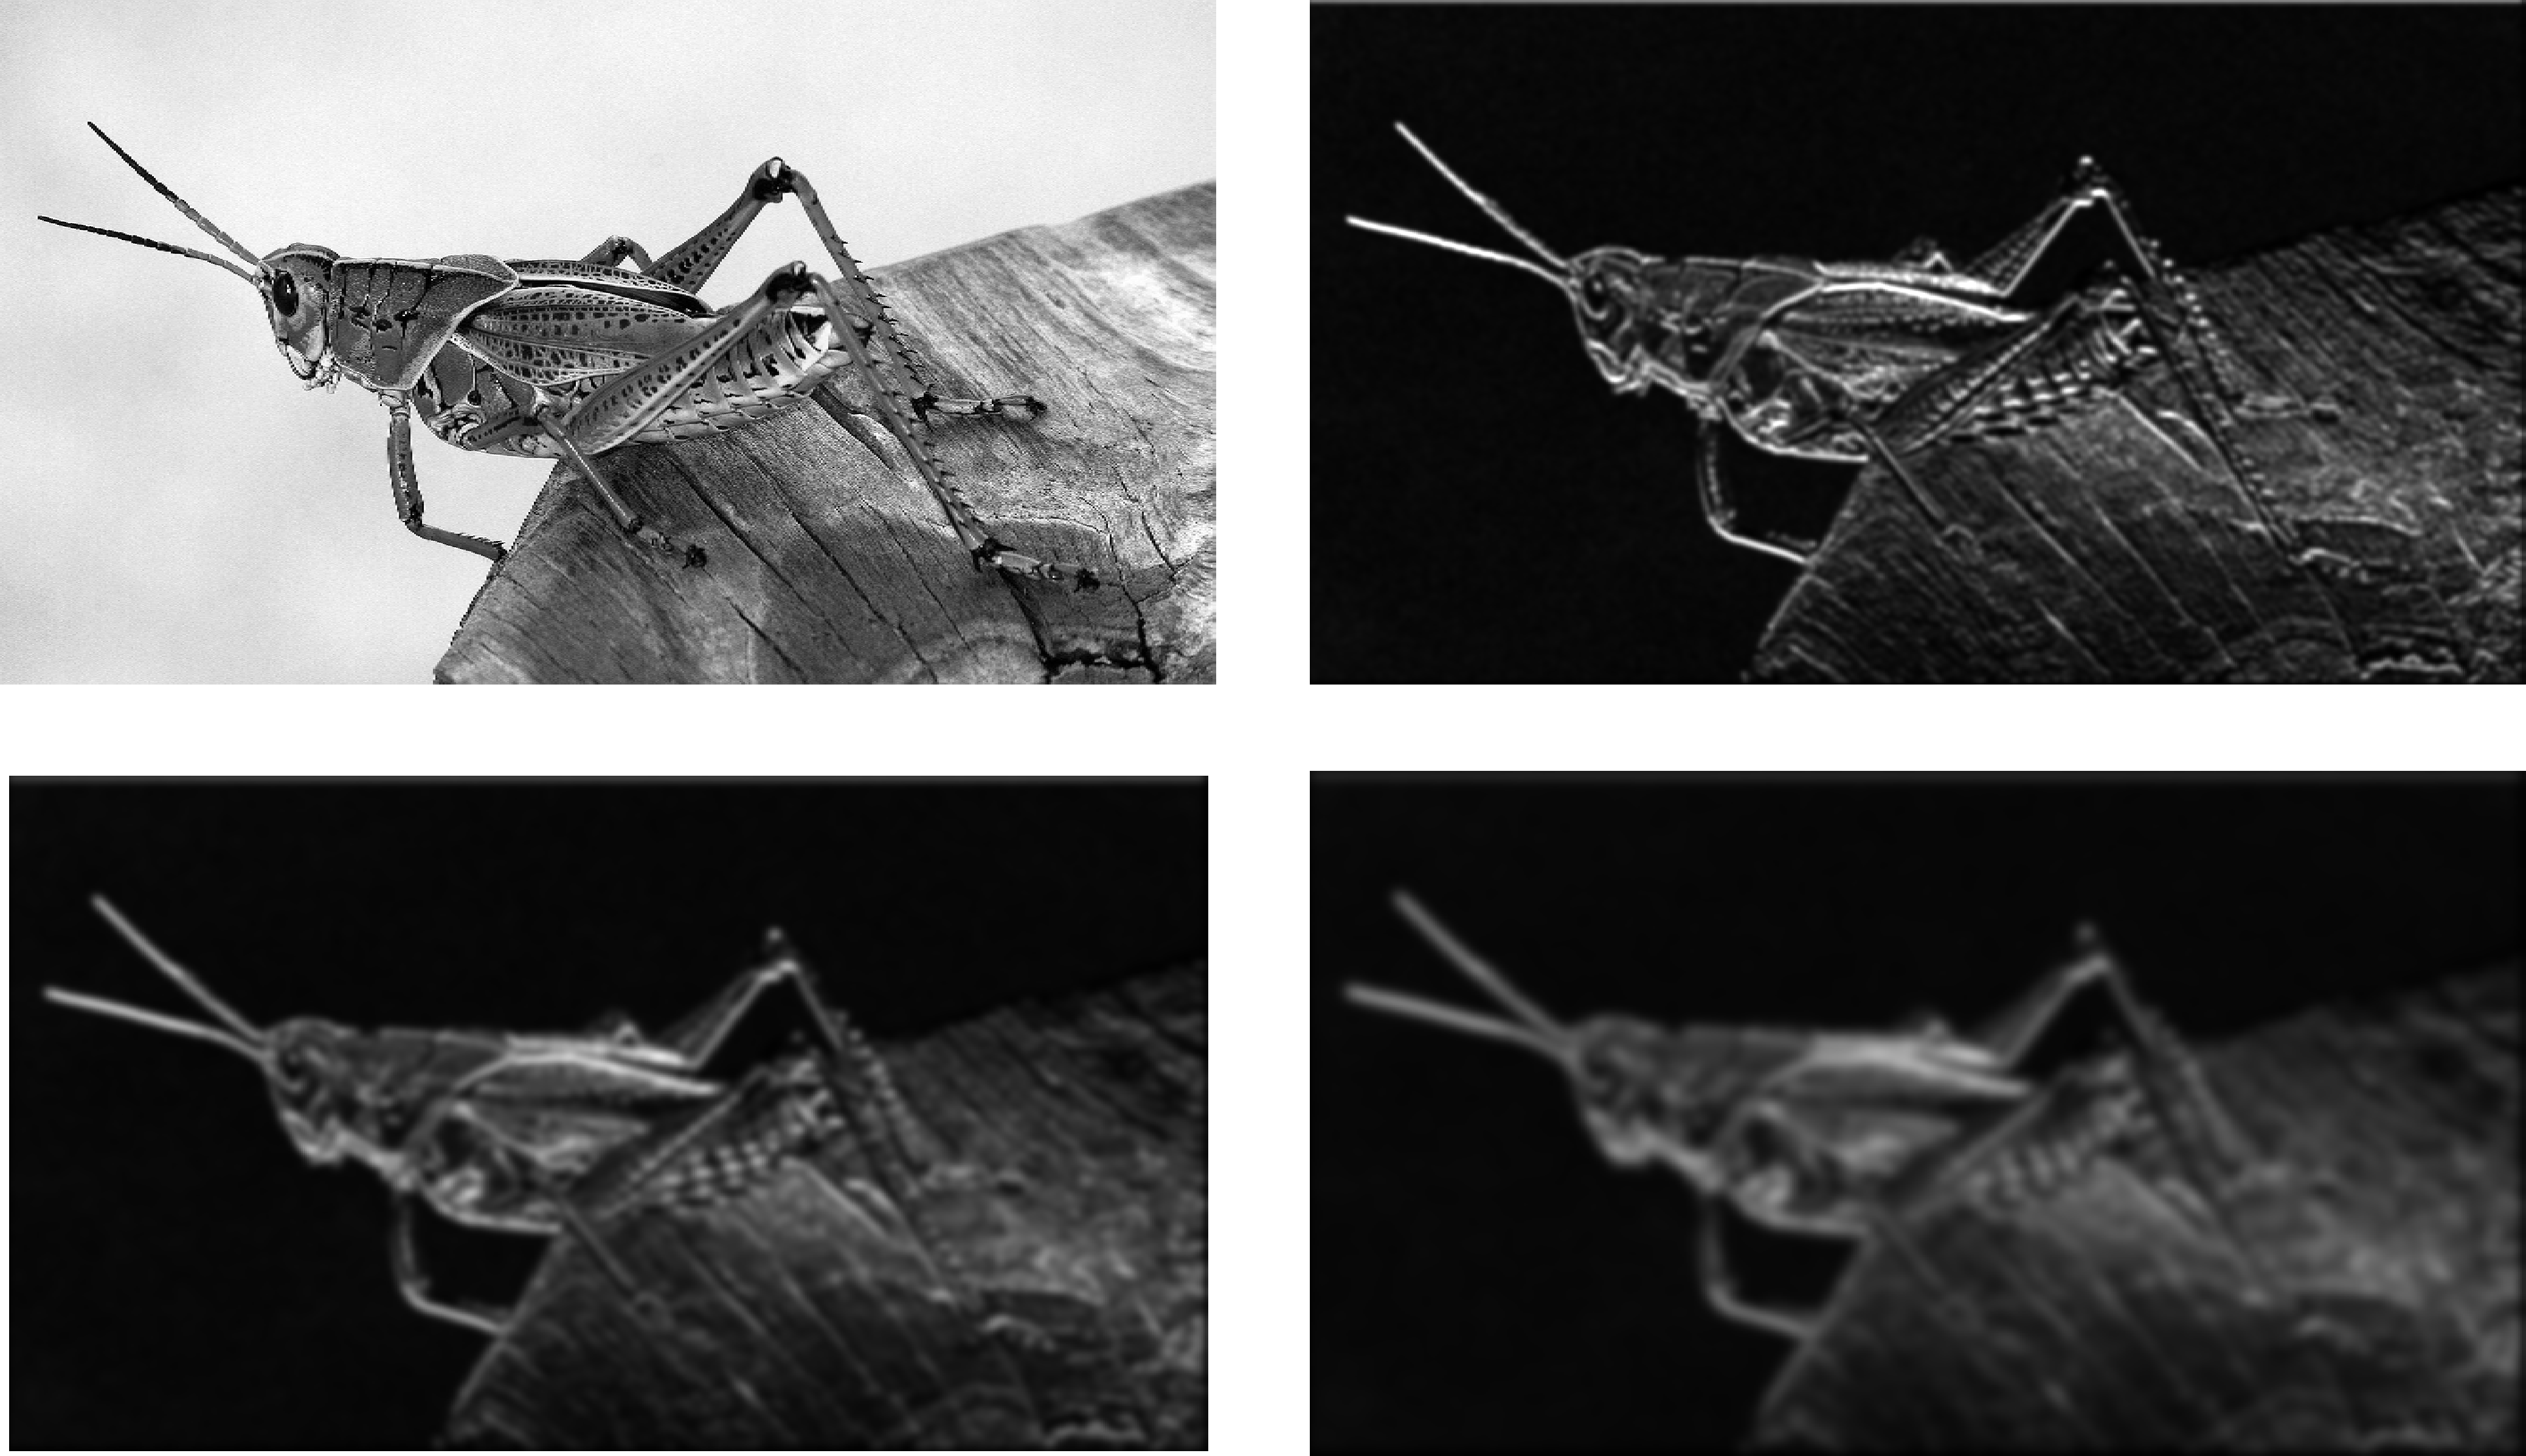
\includegraphics[width=\textwidth]{image2-table}
  \caption{Three directional derivative images and the original in the top-left
  corner}
\end{figure}

\section{Description of feature points}
